\documentclass[conference]{IEEEtran}
\IEEEoverridecommandlockouts
% The preceding line is only needed to identify funding in the first footnote. If that is unneeded, please comment it out.
\usepackage{cite}
\usepackage{amsmath,amssymb,amsfonts}
\usepackage{bm}% bold math
\usepackage{eurosym}
\usepackage{hyperref}
\usepackage{algorithmic}
\usepackage{graphicx}
\usepackage{textcomp}
\usepackage{xcolor}
\def\BibTeX{{\rm B\kern-.05em{\sc i\kern-.025em b}\kern-.08em
    T\kern-.1667em\lower.7ex\hbox{E}\kern-.125emX}}
\begin{document}

\title{\href{https://en.wikipedia.org/wiki/Quantum_computing}{\textit{Quantum Computing}:}\\
\huge{\textit{The possible growth of computing power and}\\ \textit{the consequences/repercussions that}\\ \textit{the same have on the security and privacy of users}}
}


\author{\IEEEauthorblockN{1\textsuperscript{st} Bernardo da Palma Albergaria}
\IEEEauthorblockA{\href{https://www.di.fct.unl.pt/}{\textit{Informatics Department}} \\
\href{https://www.fct.unl.pt/}{\textit{Faculty of Sciences and Technology of}} \\
\href{https://www.unl.pt/}{\textit{New University of Lisbon}}\\
\href{https://www.fct.unl.pt/}{\textit{(FCT NOVA - FCT/UNL), Portugal}}\\
        Almada, Portugal \\
        \href{mailto:bd.albergaria@campus.fct.unl.pt}{bd.albergaria@campus.fct.unl.pt}}
\and
\IEEEauthorblockN{2\textsuperscript{nd} Pedro Miguel Ribeiro}
\IEEEauthorblockA{\href{https://www.di.fct.unl.pt/}{\textit{Informatics Department}} \\
\href{https://www.fct.unl.pt/}{\textit{Faculty of Sciences and Technology of}} \\
\href{https://www.unl.pt/}{\textit{New University of Lisbon}}\\
\href{https://www.fct.unl.pt/}{\textit{(FCT NOVA - FCT/UNL), Portugal}}\\
        Almada, Portugal \\
        \href{mailto:pmg.ribeiro@campus.fct.unl.pt}{pmg.ribeiro@campus.fct.unl.pt}}
\and
\IEEEauthorblockN{3\textsuperscript{rd} R\'uben Andr\'e Barreiro}
\IEEEauthorblockA{\href{https://www.di.fct.unl.pt/}{\textit{Informatics Department}} \\
\href{https://www.fct.unl.pt/}{\textit{Faculty of Sciences and Technology of}} \\
\href{https://www.unl.pt/}{\textit{New University of Lisbon}}\\
\href{https://www.fct.unl.pt/}{\textit{(FCT NOVA - FCT/UNL), Portugal}}\\
        Almada, Portugal \\
        \href{mailto:r.barreiro@campus.fct.unl.pt}{r.barreiro@campus.fct.unl.pt}}
\and
\IEEEauthorblockN{4\textsuperscript{th} Tom\'as Ant\'onio Pessanha}
\IEEEauthorblockA{\href{https://www.di.fct.unl.pt/}{\textit{Informatics Department}} \\
\href{https://www.fct.unl.pt/}{\textit{Faculty of Sciences and Technology of}} \\
\href{https://www.unl.pt/}{\textit{New University of Lisbon}}\\
\href{https://www.fct.unl.pt/}{\textit{(FCT NOVA - FCT/UNL), Portugal}}\\
        Almada, Portugal \\
        \href{mailto:t.pessanha@campus.fct.unl.pt}{t.pessanha@campus.fct.unl.pt}}
\and
\IEEEauthorblockN{5\textsuperscript{th} Prof. Jos\'e Legatheaux Martins}
\IEEEauthorblockA{\href{https://www.di.fct.unl.pt/}{\textit{Informatics Department}} \\
\href{https://www.fct.unl.pt/}{\textit{Faculty of Sciences and Technology of}} \\
\href{https://www.unl.pt/}{\textit{New University of Lisbon}}\\
\href{https://www.fct.unl.pt/}{\textit{(FCT NOVA - FCT/UNL), Portugal}}\\
        Almada, Portugal \\
        \href{mailto:jalm@fct.unl.pt}{jalm@fct.unl.pt}}
\and
\IEEEauthorblockN{6\textsuperscript{th} Prof. Paulo Orlando Lopes}
\IEEEauthorblockA{\href{https://www.di.fct.unl.pt/}{\textit{Informatics Department}} \\
\href{https://www.fct.unl.pt/}{\textit{Faculty of Sciences and Technology of}} \\
\href{https://www.unl.pt/}{\textit{New University of Lisbon}}\\
\href{https://www.fct.unl.pt/}{\textit{(FCT NOVA - FCT/UNL), Portugal}}\\
        Almada, Portugal \\
        \href{mailto:poral@fct.unl.pt}{poral@fct.unl.pt}}
}

\maketitle
\thispagestyle{plain}
\pagestyle{plain}

\begin{abstract}
Begun in 1950s, the research for the development of the \href{https://en.wikipedia.org/wiki/Quantum_computing}{\textit{Quantum Computing}} promises to break many paradigms of \href{https://en.wikipedia.org/wiki/Von_Neumann_architecture}{\textit{Classical Computing (Von Neumann's Architecture)}}, in which can be divided into \textit{"treatable problems"} and \textit{"intractable problems"}. The recent developments in this area, also awaken some concerns in the study of \href{https://en.wikipedia.org/wiki/Internet}{\textit{Internet}}'s \href{https://en.wikipedia.org/wiki/Privacy}{Privacy} and \href{https://en.wikipedia.org/wiki/Computer_security}{\textit{Cybersecurity}}. As, the progress of research on \href{https://en.wikipedia.org/wiki/Quantum_computing}{\textit{Quantum Computing}} advances, it will bring powerful \href{https://en.wikipedia.org/wiki/Computing}{\textit{Computing}} machines with the capability of make faster computing processes and operations, and this, will take us to a huge decrease of computing process time to crack very easily some of the current most known standards and algorithms of \href{https://en.wikipedia.org/wiki/Cryptography}{\textit{Cryptography}}.
\end{abstract}

\vspace{4pt}

\begin{IEEEkeywords}
\href{https://en.wikipedia.org/wiki/Quantum_computing}{Quantum Computing}, \href{https://en.wikipedia.org/wiki/Cryptography}{Cryptography}, \href{https://en.wikipedia.org/wiki/Computer_security}{Cybersecurity}, \href{https://en.wikipedia.org/wiki/Internet}{Internet}, \href{https://en.wikipedia.org/wiki/Privacy}{Privacy}
\end{IEEEkeywords}

\vspace{6pt}

\section{Introduction}
This article/paper will focus in the evolution of the history's timeline of the \href{https://en.wikipedia.org/wiki/Quantum_computing}{\textit{Quantum Computing}} in world's society, focusing more in its application on Internet's security and privacy, as also, the benefits and concerns to the \href{https://en.wikipedia.org/wiki/Cryptography}{\textit{Cryptography}} and \href{https://en.wikipedia.org/wiki/Computer_security}{\textit{Cybersecurity}}.

\vspace{6pt}

\section{Timeline and History}

\subsection{The Beginning of the \href{https://en.wikipedia.org/wiki/Quantum_computing}{Quantum Computing} and its history over the years}\label{AA}

The research for the development of the \href{https://en.wikipedia.org/wiki/Quantum_computing}{\textit{Quantum Computing}} began as early as the 1950s when was thought in the application of the laws of \href{https://en.wikipedia.org/wiki/Physics}{\textit{Physics}} and \href{https://en.wikipedia.org/wiki/Quantum_mechanics}{\textit{Quantum Mechanics}} to computers.

\newpage

In 1981 at a conference at \href{https://en.wikipedia.org/wiki/Massachusetts_Institute_of_Technology}{\textit{MIT}}, the \href{https://en.wikipedia.org/wiki/Richard_Feynman}{\textit{Physicist Richard Feynman}} presented a proposal for using \href{https://en.wikipedia.org/wiki/Quantum_system}{\textit{Quantum Systems}} in \href{https://en.wikipedia.org/wiki/Computer}{\textit{Computers}}, which would then have a higher processing capacity than ordinary \href{https://en.wikipedia.org/wiki/Computer}{\textit{Computers}}.

\vspace{4pt}

As early as 1985, \href{https://en.wikipedia.org/wiki/David_Deutsch}{\textit{David Deutsch}} of \href{https://en.wikipedia.org/wiki/University_of_Oxford}{\textit{University of Oxford}} described the first \href{https://en.wikipedia.org/wiki/Quantum_computing}{\textit{Quantum Computer}}, a \textit{Quantum Turing Machine}, it would simulate another \href{https://en.wikipedia.org/wiki/Quantum_computing}{\textit{Quantum Computer}}.

\vspace{4pt}

In 1994, at \href{https://en.wikipedia.org/wiki/Bell_Labs}{\textit{AT} \& \textit{T Bell Labs}}, in \href{https://en.wikipedia.org/wiki/New_Jersey}{\textit{New Jersey}}, the \href{https://en.wikipedia.org/wiki/Applied_mathematics}{\textit{Applied Mathematics}}' Professor \href{https://en.wikipedia.org/wiki/Peter_Shor}{\textit{Peter Shor}} developed the \href{https://en.wikipedia.org/wiki/Shor\%27s_algorithm}{\textit{Shor's Algorithm}}, capable of factoring large numbers at a much faster speed than \href{https://en.wikipedia.org/wiki/Von_Neumann_architecture}{\textit{conventional computers}}.

\vspace{4pt}

In 1996, \href{https://en.wikipedia.org/wiki/Lov_Grover}{\textit{Lov Grover}}, also of \href{https://en.wikipedia.org/wiki/Bell_Labs}{\textit{Bell Labs}}, developed \href{https://en.wikipedia.org/wiki/Amdahl\%27s_law}{\textit{Speedup}}, the first algorithm for \textit{Quantum Database Research}. In that same year, a model for the \href{https://en.wikipedia.org/wiki/Quantum_error_correction}{\textit{correction of the Quantum Error}} was proposed.

\vspace{4pt}

In 1999, at \href{https://en.wikipedia.org/wiki/Massachusetts_Institute_of_Technology}{\textit{MIT}}, the first prototypes of \href{https://en.wikipedia.org/wiki/Quantum_computing}{\textit{Quantum Computer}} were built using thermal assembly.

\vspace{4pt}

In 2007, was developed by the Canadian company \href{https://en.wikipedia.org/wiki/D-Wave_Systems}{\textit{D-Wave Systems}}, a \href{https://en.wikipedia.org/wiki/Quantum}{\textit{Quantum}} 16 \href{https://en.wikipedia.org/wiki/Qubit}{\textit{qubits}} \href{https://en.wikipedia.org/wiki/Processor_(computing)}{processor} called \href{https://www.eetimes.com/document.asp?doc_id=1165219#}{\textit{Orion}} that performs practical tasks.

\vspace{4pt}

In 2011, \href{https://en.wikipedia.org/wiki/D-Wave_Systems}{\textit{D-Wave Systems}} launched the first \href{https://en.wikipedia.org/wiki/Quantum_computing}{\textit{Quantum Computer}} for commercialization, the \textit{D-Wave One}, which has a \textit{128-\href{https://en.wikipedia.org/wiki/Qubit}{qubit} \href{https://en.wikipedia.org/wiki/Processor_(computing)}{processor}}. But the \href{https://en.wikipedia.org/wiki/D-Wave_Systems#D-Wave_One}{\textit{D-Wave One}} isn't yet fully independent, it needs to be used in conjunction with \href{https://en.wikipedia.org/wiki/Von_Neumann_architecture}{\textit{conventional computers}}.

\vspace{4pt}

In 2017, \href{https://en.wikipedia.org/wiki/D-Wave_Systems}{\textit{D-Wave Systems}} commercially launched the \href{https://www.dwavesys.com/d-wave-two-system}{\textit{2000Q}}, a \href{https://en.wikipedia.org/wiki/Quantum_computing}{\textit{Quantum Computer}} of 2,000 \href{https://en.wikipedia.org/wiki/Qubit}{\textit{qubits}} at a meager \$ 15 million. The company's previous \href{https://en.wikipedia.org/wiki/Quantum_computing}{\textit{Quantum Computer}} had 1,000 \href{https://en.wikipedia.org/wiki/Qubit}{\textit{qubits}}. The \href{https://www.dwavesys.com/d-wave-two-system}{\textit{D-Wave Systems' 2000Q}} is capable to perform 2,2000 operations at the same time.

\vspace{4pt}

In 2017, \href{https://www.researchgate.net/profile/Guilherme_Tosi}{\textit{Guilherme Tosi}} and a team of researchers from the \href{https://en.wikipedia.org/wiki/University_of_New_South_Wales}{\textit{University of New South Wales}}, invented a radical new architecture for \href{https://en.wikipedia.org/wiki/Quantum_computing}{\textit{Quantum Computing}}, based on \href{https://phys.org/news/2017-09-flip-flop-qubits-radical-quantum.html}{\textit{"flip-flop qubits"}} that can be used in a new type of \href{https://en.wikipedia.org/wiki/Quantum_computing}{\textit{Quantum Computers}} thus enabling the manufacture of large-scale \href{https://en.wikipedia.org/wiki/Quantum}{\textit{Quantum}} \href{https://en.wikipedia.org/wiki/Processor_(computing)}{\textit{processors}} can become much cheaper and easier than was thought possible.

\vspace{4pt}

In 2017, \href{https://en.wikipedia.org/wiki/IBM}{\textit{IBM}} announced a \href{https://en.wikipedia.org/wiki/Quantum_computing}{\textit{Quantum Computer}} that handles 50 \href{https://en.wikipedia.org/wiki/Qubit}{\textit{qubits}}. The company is also making a 20-\href{https://en.wikipedia.org/wiki/Qubit}{\textit{qubit}} system available through its \href{https://en.wikipedia.org/wiki/Cloud_computing}{\textit{Cloud Computing}} platform.

\vspace{4pt}

In 2018, at the \href{https://www.aps.org/meetings/meeting.cfm?name=MAR18}{\textit{APS March 2018 Conference}}, \href{https://en.wikipedia.org/wiki/Google}{\textit{Google}} announced it has created a 72 \href{https://en.wikipedia.org/wiki/Qubit}{\textit{qubits}} chip called \href{https://ai.googleblog.com/2018/03/a-preview-of-bristlecone-googles-new.html}{\textit{Bristlecone}} which will serve as a basis for its demonstration of \href{https://en.wikipedia.org/wiki/Quantum}{\textit{Quantum}} supremacy.

\vspace{4pt}

In 2019, at \href{https://en.wikipedia.org/wiki/New_York_City}{\textit{New York}}, \href{https://en.wikipedia.org/wiki/IBM}{\textit{IBM}} unveiled \href{https://en.wikipedia.org/wiki/IBM_Q_System_One}{\textit{IBM Q System One\texttrademark}}, the world's first integrated universal approximate \href{https://en.wikipedia.org/wiki/Quantum_computing}{\textit{Quantum Computer System}} designed for scientific and commercial use. \href{https://en.wikipedia.org/wiki/IBM}{\textit{IBM}} also announced plans to open its first \href{https://www.research.ibm.com/ibm-q/}{\textit{IBM Q Quantum Computation Center}} for commercial clients, also in \href{https://en.wikipedia.org/wiki/New_York_City}{\textit{New York}}.

\vspace{4pt}

In 2019, a team of \href{https://en.wikipedia.org/wiki/Physicist}{Physicists} from \href{https://en.wikipedia.org/wiki/United_States}{\textit{U.S.A.}}, \href{https://en.wikipedia.org/wiki/Russia}{\textit{Russia}} and \href{https://en.wikipedia.org/wiki/Switzerland}{\textit{Switzerland}}, led by \href{https://www.researchgate.net/profile/Gordey_Lesovik}{\textit{Gordey Lesovik}}, \href{https://www.researchgate.net/profile/Andrey_Lebedev4}{\textit{Andrei Lebedev}} and \href{https://www.researchgate.net/profile/Henning_Bostelmann}{\textit{Henning Bostelmann}}, \href{https://en.wikipedia.org/wiki/Electron}{\textit{"experimentally demonstrate a time reversal"}} in a single \href{https://en.wikipedia.org/wiki/Electron}{\textit{electron}}, sending a \href{https://en.wikipedia.org/wiki/Qubit}{\textit{qubit}} from a more complicated state to a simpler one. The experiment's results from the \href{https://www.researchgate.net/publication/322160389_Arrow_of_time_and_its_reversal_on_IBM_quantum_computer}{\textit{"reversal algorithm"}} got a success rate of 85\% in a \href{https://en.wikipedia.org/wiki/Quantum_computing}{\textit{Quantum Computer}} of 2 \href{https://en.wikipedia.org/wiki/Qubit}{\textit{qubits}}, occurring more errors and dropping to a success rate to 50\%, when introduced a 3rd \href{https://en.wikipedia.org/wiki/Qubit}{\textit{qubit}}.

\vspace{6pt}

\subsection{Principles of \href{https://en.wikipedia.org/wiki/Quantum_computing}{Quantum Computing}}\label{AA}

The \href{https://en.wikipedia.org/wiki/Quantum_computing}{\textit{Quantum Computing}} promises to break many paradigms of \textit{Classical Computing}, in which we can divide the problems into \href{http://www.cs.ucc.ie/~dgb/courses/toc/handout29.pdf}{\textit{"tractable problems"}}, that are problems that have reasonable, polynomial-time solutions and \href{http://www.cs.ucc.ie/~dgb/courses/toc/handout29.pdf}{\textit{"intractable problems"}}, that are problems that don't have it:

\begin{table}[!hp]
\centering
    \caption{Tractable and Intractable Problems in Classical Computing}
    \begin{tabular}{ |p{2.2cm}|p{3cm}|p{2.2cm}| }
     \hline
     \begin{center}\textbf{\textit{Mathematical Notation}}\end{center} & \begin{center}\textbf{\textit{Complexity Time}}\end{center} & \begin{center}\textbf{\textit{Tractable/\\Intractable}}\end{center}\\
     \hline
     \hline
     \textbf{O(1)} & Constant & \textbf{Tractable} \\
     \hline
     $\bm{O(\log(n))}$ & Logarithmic & \textbf{Tractable} \\
     \hline
     \textbf{O(n)} & Linear & \textbf{Tractable} \\
     \hline
     $\bm{O(n\times\log(n))}$ & N-Log-N & \textbf{Tractable} \\
     \hline
     \textbf{O(n$^{2}$)} & Polynomial (Quadratic) & \textbf{Tractable} \\
     \hline
     \textbf{O(n$^{3}$)} & Polynomial (Cubic) & \textbf{Tractable} \\
     \hline
     \hline
     \textbf{O(k$^{n}$), e.g., O(2$^{n}$)} & Exponential & \textbf{Intractable} \\
     \hline
     \textbf{O(n!)} & Factorial & \textbf{Intractable} \\
     \hline
     \textbf{O(n$^{n}$)} & Super-Exponential & \textbf{Intractable} \\
     \hline
    \end{tabular}
\end{table}


\newpage

All the elements that change the \href{https://en.wikipedia.org/wiki/Structure_and_Interpretation_of_Classical_Mechanics}{\textit{Classical Structures}} come from the changes that \href{https://en.wikipedia.org/wiki/Classical_physics}{\textit{Classical Physics}} has brought. \href{https://en.wikipedia.org/wiki/Physicist}{Physicists} like \href{https://en.wikipedia.org/wiki/Werner_Heisenberg}{\textit{Heisenberg}}, \href{https://en.wikipedia.org/wiki/Niels_Bohr}{\textit{Bohr}}, \href{https://en.wikipedia.org/wiki/Erwin_Schr\%C3\%B6dinger}{\textit{Schr\"odinger}}, and \href{https://en.wikipedia.org/wiki/Albert_Einstein}{\textit{Einstein}} studied these new foundations. Among them, it can be highlighted:

\vspace{6pt}

\begin{itemize}
  \item \textit{Quantum Overlap}:
    \begin{itemize}
        \item The \textit{Quantum Overlap} is a fundamental principle of \href{https://en.wikipedia.org/wiki/Quantum_mechanics}{\textit{Quantum Mechanics}} that states that a \href{https://en.wikipedia.org/wiki/Physical_system}{\textit{Physical System}} exists partially in all theoretically possible states simultaneously before being measured. But when measured or observed, the system is shown in a single state;
    \end{itemize}
  
  \vspace{4pt}
  
  \item \href{https://en.wikipedia.org/wiki/Schr\%C3\%B6dinger\%27s_cat}{\textit{Schr\"odinger's Cat Experience}}:
    \begin{itemize}
        \item The \href{https://en.wikipedia.org/wiki/Schr\%C3\%B6dinger\%27s_cat}{\textit{Schr\"odinger's Cat}} is a mental experiment, often described as a paradox, developed by \href{https://en.wikipedia.org/wiki/Erwin_Schr\%C3\%B6dinger}{\textit{Erwin Schr\"odinger}}, in 1935. The experiment seeks to illustrate Copenhagen's interpretation of \href{https://en.wikipedia.org/wiki/Quantum_mechanics}{\textit{Quantum Mechanics}} by imagining it applied to everyday objects. In the example, there is a cat enclosed in a box, so that it is not only alive or only dead, but "undead";
    \end{itemize}
  \begin{center}
      \begin{figure}[htbp]
        \centerline{\href{https://en.wikipedia.org/wiki/Schr\%C3\%B6dinger\%27s_cat}{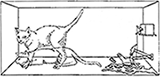
\includegraphics{fig1.png}}}
        \caption{The \href{https://en.wikipedia.org/wiki/Schr\%C3\%B6dinger\%27s_cat}{\textit{Schr\"odinger's Cat Experience}}.}
        \label{fig}
      \end{figure}
  \end{center}
 
  \item \href{https://en.wikipedia.org/wiki/Quantum_entanglement}{\textit{Quantum Entanglement} or \\\textit{"Ghostly Action at a Distance"}}:
   
    \begin{itemize}
        \item The \href{https://en.wikipedia.org/wiki/Quantum_entanglement}{\textit{Quantum Entanglement}} is a phenomenon of \href{https://en.wikipedia.org/wiki/Quantum_mechanics}{\textit{Quantum Mechanics}} that allows two or more objects to be somehow so connected that an object can't be correctly described without its counterpart be mentioned (even though the objects may be spatially separated by millions of light years). This leads to very strong correlations between the observable physical properties of the various subatomic particles. The \href{https://en.wikipedia.org/wiki/Quantum_entanglement}{\textit{Quantum Entanglement}} was called \href{https://en.wikipedia.org/wiki/Quantum_entanglement}{\textit{"Ghostly Action at a Distance"}} by \href{https://en.wikipedia.org/wiki/Albert_Einstein}{\textit{Albert Einstein}}, who believed it to be an impossible event under the laws of orthodox \href{https://en.wikipedia.org/wiki/Quantum_mechanics}{\textit{Quantum Mechanics}};
    \end{itemize}
    \begin{center}
      \begin{figure}[htbp]
        \centerline{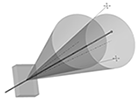
\includegraphics{fig2.png}}
        \caption{How Quantum Entanglement works.}
        \label{fig}
      \end{figure}
  \end{center}
  
\end{itemize}

\newpage

\begin{itemize}
  \item \href{https://en.wikipedia.org/wiki/Quantum_teleportation}{\textit{Quantum Teleportation}}:
    \begin{itemize}
        \item The \href{https://en.wikipedia.org/wiki/Quantum_teleportation}{\textit{Quantum Teleportation}} is a technology that allows teleportation of information, such as spin or polarization (there's no transport of energy or matter) by exclusively \href{https://en.wikipedia.org/wiki/Quantum}{\textit{Quantum}} means, which are independent of transmission media. The bandwidth for \href{https://en.wikipedia.org/wiki/Quantum_teleportation}{\textit{Quantum Teleportation}} doubled in 2015. It's a Chinese technique of transferring information about one particle so that another particle takes two instead of just one of the \href{https://en.wikipedia.org/wiki/Quantum}{\textit{Quantum}} properties of the initial particle;
    \end{itemize}

  \vspace{4pt}

  \item \href{https://en.wikipedia.org/wiki/Rutherford_scattering}{\textit{Rutherford Scattering}}:
    \begin{itemize}
        \item In \href{https://en.wikipedia.org/wiki/Physics}{Physics}, \href{https://en.wikipedia.org/wiki/Rutherford_scattering}{\textit{Rutherford's Dispersion}} is a phenomenon that was explained by \href{https://en.wikipedia.org/wiki/Ernest_Rutherford}{\textit{Ernest Rutherford}}, in 1909, and led to the development of the \href{https://en.wikipedia.org/wiki/Atomic_orbital}{\textit{orbital theory of the atom}}. It's now exploited by the \href{https://en.wikipedia.org/wiki/Rutherford_scattering}{\textit{Rutherford's Dispersion Spectrometry Material Analysis}} technique. The \href{https://en.wikipedia.org/wiki/Rutherford_scattering}{\textit{Rutherford's Dispersion}} is also sometimes referred to as \href{https://en.wikipedia.org/wiki/Rutherford_scattering}{\textit{Coulomb's Dispersion}} because it is based on \href{https://en.wikipedia.org/wiki/Electrostatics}{\textit{Electrostatic Forces}} (\href{https://en.wikipedia.org/wiki/Coulomb\%27s_law}{\textit{Coulomb}}). A similar process proved the core interior in the 1960s, called \href{https://arxiv.org/abs/1601.05453}{\textit{Inelastic Deep Dispersion}};
    \end{itemize}
  \item \textit{Existence of Multiverse}:
    \begin{itemize}
        \item The \href{https://en.wikipedia.org/wiki/Many-worlds_interpretation}{\textit{Quantum Multiverse}} (also known as \href{https://en.wikipedia.org/wiki/Many-worlds_interpretation}{\textit{Multiverse Theory}} or \href{https://en.wikipedia.org/wiki/Many-worlds_interpretation}{\textit{Many-worlds' Interpretation}}) is an interpretation of \href{https://en.wikipedia.org/wiki/Quantum_mechanics}{\textit{Quantum Mechanics}} that asserts the objective reality of the universal wave-function and denies the actuality of wave-function collapse. The existence of the other worlds makes it possible to remove randomness and action at a distance from \href{https://en.wikipedia.org/wiki/Quantum_theory}{\textit{Quantum Theory}} and thus from all \href{https://en.wikipedia.org/wiki/Physics}{\textit{Physics}}. The \href{https://en.wikipedia.org/wiki/Many-worlds_interpretation}{\textit{Quantum Multiverse}} implies that all possible alternate histories and futures are real, each representing an actual "world" (or "universe");
    \end{itemize}
\end{itemize}

\vspace{6pt}

And it was thanks to these principles that the development of \href{https://en.wikipedia.org/wiki/Quantum_computing}{\textit{Quantum Computing}} was possible.

\vspace{6pt}

\section{Learning \href{https://en.wikipedia.org/wiki/Quantum}{Quantum}}

\subsection{Understanding the \href{https://en.wikipedia.org/wiki/Quantum_computing}{\textit{Quantum Computing}}}\label{AA}

The \href{https://en.wikipedia.org/wiki/Quantum_mechanics}{\textit{Quantum Mechanics}} is considered to be the most successful \textit{Physical Theory}. For from its creation to the present day, it has been applied in diverse branches, from \textit{Particle Physics}, \textit{Atomic and Molecular to Astrophysics} and \textit{Condensed Matter}.

\vspace{4pt}

In \href{https://en.wikipedia.org/wiki/Quantum_computing}{\textit{Quantum Computing}}, the basic information unit is the \textit{Quantum Bit} or \textit{Qubit}. The fact that \textit{Quantum Computing} it's so powerful lies in the fact that in addition to assuming zero ('\textbf{0}') and one ('\textbf{1}'), as in \href{https://en.wikipedia.org/wiki/Von_Neumann_architecture}{\textit{Classical Computing}}'s memory (following the \href{https://en.wikipedia.org/wiki/Von_Neumann_architecture}{\textit{Von Neumann's Architecture}}) made up of \textit{bits}, it can assume both zero ('\textbf{0}') and one ('\textbf{1}') states at the same time by \textit{Quantum Superposition} of those 2 \textit{qubit} states.

\newpage

A pair of \textit{qubits} can be in any \textit{Quantum Superposition} of 4 states, and three \textit{qubits} in any superposition of 8 states. In general, a \textit{Quantum Computer} with \textit{n qubits} can be in any superposition of up to 2\textsuperscript{n} different states (this compares to a normal computer that can only be in one of these 2\textsuperscript{n} states at any one time).

\vspace{4pt}

It's hard to assume the two different states at the same time, but \textit{Schr\"odinger's Cat's Mental Experience} can give an intuitive sense to the situation. And it's thanks to this property of the \textit{Quantum Superposition} of states that motivated the studies in \textit{Quantum Computing}. If in \textit{Classical Computing}, the processing is sequential, in the \textit{Quantum Computing}, the processing is simultaneous.

\vspace{4pt}

The \textit{qubit} is described by a states' vector in a two-level \textit{Quantum System}, which is equivalent to a two-dimensional space's vector over complex numbers. The \textit{bra-ket}'s notation is used to represent them:

\vspace{4pt}

\begin{itemize}
    \item 
    \begin{center}
        $\mid$\textbf{0}$\rangle$ = ${
            \begin{bmatrix}
                \textbf{0}\\
                \textbf{1}
            \end{bmatrix}}$ 
        or even, 
        $\mid$\textbf{1}$\rangle$ = ${
            \begin{bmatrix}
                \textbf{0}\\
                \textbf{1}
            \end{bmatrix}}$ 
    \end{center}
\end{itemize}

\vspace{4pt}

Thus, the state of a \textit{qubit} can be represented by:

\vspace{4pt}

\begin{itemize}
    \item 
    \begin{center}
        $\mid$$\psi$$\rangle$ = $\alpha$$\mid$\textbf{0}$\rangle$ + $\beta$$\mid$\textbf{1}$\rangle$
    \end{center}
\end{itemize}

\vspace{4pt}

The set \{$\mid$0$\rangle$, $\mid$1$\rangle$\} forms a two-dimensional \textit{Hilbert's Space} called the \textit{Computational Basis}.

\vspace{4pt}

For the manipulation of \textit{Quantum States}, some kind of \textit{Optical Techniques}, \textit{i.e.}, \textit{Electromagnetic Radiation}, are used. These devices constitute \textit{Quantum Logic Gates}. A \textit{Quantum Computer} operates on its \textit{qubits} using this \textit{Quantum Logic Gates} and measurement (which also alters the observed state). This manipulation can be performed using \textit{atoms} that can be excited or not, or even, the both, at the same time.

\vspace{4pt}

Another device used is the manipulation of \textit{photons}. The advantage of using them lies in the fact that these \textit{photons} can constitute highly stable carriers of \textit{Quantum Information}.

\vspace{4pt}

However, \textit{photons} don't interact directly with each other, requiring the use of an \textit{atom} as a mediator, which introduces additional noise and complications in the experiments. In this case, a \textit{photon} interacts with an \textit{atom} which in turn interacts with the second \textit{photon}, leading to the complete interaction between the two \textit{photons}.

\vspace{4pt}

 A \textit{Quantum Algorithm} is composed of a fixed sequence of \textit{Quantum Logic Gates} and a problem is encoded by setting the initial values of the \textit{qubits}, similar to how a \textit{Classical Computer} works.
 
 \vspace{4pt}
 
 The calculation usually ends with a measurement, collapsing the system of \textit{qubits} into one of the 2\textsuperscript{n} \textit{eigenstates}, where each \textit{qubit} is zero ('\textbf{0}') or one ('\textbf{1}'), decomposing into a classical state. The outcome can, therefore, be at most \textit{n} classical \textit{bits} of information. If the algorithm didn't end with a measurement, the result is an unobserved \textit{Quantum State} (such unobserved states may be sent to other computers as part of \textit{Distributed Quantum Algorithms}).

\newpage

The \textit{Quantum Algorithms} are often probabilistic, in that they provide the correct solution only with a certain known probability. Note that the term \textit{non-deterministic computing} mustn't be used in that case to mean probabilistic (computing) because the term non-deterministic has a different meaning in \textit{Computer Science} and \textit{Informatics}.

\vspace{4pt}

In order to store the \textit{qubits}, \textit{ion's traps} are used, in which a small number of charged \textit{atoms} are trapped, and also, \textit{neutral ion's traps} to trap uncharged \textit{atoms}.

\vspace{4pt}

In this scheme, the \textit{photons} are used to manipulate the information contained in the \textit{atoms}, in this way they constitute a type of \textit{Quantum Logic Gate} that applies appropriate \textit{pulses of electromagnetic radiation} so that the \textit{atoms} in the neighborhood can interact with each other like via, per example, \textit{dipole forces}.

\vspace{4pt}

Another class of \textit{Quantum Information Processing} is based on \textit{Nuclear Magnetic Resonance} (\textit{N.M.R.}). In this case, the \textit{Quantum Information} is stored in the \textit{nuclear spins} of the \textit{atoms} in \textit{molecules} and the \textit{Quantum Logical Gates} manipulate that information using the \textit{electromagnetic radiation}.

\vspace{4pt}

This is an example of an implementation of \textit{qubits} in a \textit{Quantum Computer}, where could start with the use of \textit{particles} (\textit{electrons}) with two spin states: \textit{"down"} and \textit{"up"}, as also, the both at the same time (typically written \textbf{$\mid\downarrow\rangle$} and \textbf{$\mid\uparrow\rangle$}, or \textbf{$\mid$0$\rangle$} and \textbf{$\mid$1$\rangle$}). This is true because any such system can be mapped onto an effective \textit{spin-$\frac{1}{2}$ system}.

\vspace{4pt}

The \textit{nuclear magnetic moments} make a \textit{natural precession movement} in the presence of \textit{magnetic fields}. The \textit{Quantum States} of the cores can be manipulated by irradiating the cores with \textit{radio frequency pulses} tuned to the \textit{precession frequency} of these.

\vspace{4pt}

In a given compound made up of different atoms one can measure the resonances of the cores of some \textit{atoms} without altering them, using \textit{Nuclear Magnetic Resonance} (\textit{N.M.R.}). It's sensitive to the interactions of the \textit{nuclear moments} exposed to the \textit{local electric} and \textit{magnetic fields}, these interactions are called \textit{hyper-fines}. Each type of spin has an angular velocity that depends on the applied field and the exchange interaction between them.

\begin{figure}[htbp]
\centerline{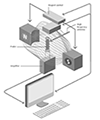
\includegraphics{fig3.png}}
\caption{Nuclear Magnetic Resonance (N.M.R.).}
\label{fig}
\end{figure}

\newpage

Just as in \textit{Classical Computing}, in \textit{Quantum Computing} are used \textit{Circuits}, but these \textit{Circuits} are \textit{Quantum}:

\vspace{4pt}

\begin{itemize}
    \item \textbf{Input}: \textit{The input qubits are considered together, mathematically what is called their tensor product};
    \item \textbf{Horizontal Lines}: \textit{The lines that appear aren't necessarily wires. They represent the evolution of a qubit, which may be only the passage of time or, for example, the displacement of a photon};
    \item \textbf{Direction}: \textit{The circuit describes the evolution of the quantum system in time, from left to right};
    \item \textbf{Vertical Lines}:
    \begin{itemize}
        \item \textit{The vertical segment informs that the circuit acts simultaneously on both qubits. The vertical line represents the synchronization, not the sending of information};
    \end{itemize}
    \item \textbf{Control}:
    \begin{itemize}
        \item \textit{Indicates that the qubit represented in this line is a control qubit, that is}:
        \begin{itemize}
            \item \textit{If it's in the \textbf{$\mid$1$\rangle$} state, the port performs the operation};
            \item \textit{If it's in the \textbf{$\mid$0$\rangle$} state, the port doesn't \\perform any operation};
            \item \textit{If the control qubit is a superposed state or the 2 qubits are entangled, it's not possible to understand the individual behavior of the control qubit and the target qubit};
            \item \textit{Must be considered the action of \\the unit operator, which represents the \\entire circuit, acting simultaneously \\on the 2 qubits};
        \end{itemize}
    \end{itemize}
    \item \textbf{Output}:
    \begin{itemize}
        \item \textit{The qubits that make up the circuit output may or may not be measured};
        \item \textit{As the lower qubit is being measured, the result will be zero ('\textbf{0}') or one ('\textbf{1}')};
    \end{itemize}
\end{itemize}

\vspace{4pt}

So, \textit{logical operations} or even \textit{algorithms}, can be described by a \textit{Quantum Circuit}. In these \textit{Circuits}, can be used the \textit{Logic Gates} used in \textit{Classical Computing}, but it's possible to use others that may allow, per example, the construction of a \textit{possible circuit for the teleportation of data}.

\vspace{4pt}

However, in the same way that, the property of \textit{Superposition of States} allows the creation of the \textit{Quantum Computer}, it's this same property that makes it impossible to create them.

\vspace{4pt}

The \textit{Superposition of States} is very sensitive to any \textit{electromagnetic micro-disturbance} that can alter the state of the \textit{qubit} causing the information contained in it to be lost.

\vspace{4pt}

Another important fact in question is the \textit{overheating of the machines}. It's for that reason that it's almost mandatory use this kind of systems cooled with temperatures closer to \textit{"absolute zero"}.

\newpage

Actually, it's possible to perform any \textit{classical operation} using only \textit{\textbf{NAND}} ports. The same occurs in \textit{Quantum Circuits} where the ports are:

\begin{itemize}
    \item Hadanard (H)
    \item Controller (CNOT)
    \item Phase (S)
    \item $\frac{\pi}{8}$(T)
\end{itemize}

\vspace{4pt}

Some examples of \textit{Quantum} ports are:

\begin{itemize}
    \item \textit{Quantum} \textit{\textbf{NOT}} port:
    \begin{itemize}
        \item In the \textit{classic} case, the \textit{\textbf{NOT}} port changes the zero ('0') by one ('1'), and vice versa;
        \item The generalization for the \textit{Quantum} case is given by an operator \textit{\textbf{X}} that satisfies:
        
        \vspace{4pt}
        
        \begin{itemize}
            \item 
            \begin{center}
                \textbf{
                    \textit{X}$\mid$1$\rangle$ = $\mid$0$\rangle$ and \textit{X}$\mid$0$\rangle$ = $\mid$1$\rangle$
                }
            \end{center}
        \end{itemize}
        
        \vspace{4pt}
        
        \item With this, it's easy to verify that the matrix representation of the operator \textit{\textbf{X}} is given by:
        
        \vspace{4pt}
        
        \begin{itemize}
            \item 
            \begin{center}
                \textbf{
                    \textit{X} = ${
                    \begin{bmatrix}
                        \textbf{0} & \textbf{1}\\
                        \textbf{1} & \textbf{0}
                    \end{bmatrix}}$
                }
            \end{center}
        \end{itemize}
        
        \vspace{4pt}
        
        \item With the \textit{Quantum} \textit{\textbf{NOT}} port, there are unmatched situations in the \textit{classical case}, because if the input $\mid$$\phi$$\rangle$ is a \textit{Quantum Superposition} of the states $\mid$0$\rangle$ and $\mid$1$\rangle$:
        
        \vspace{4pt}
        
        \begin{itemize}
            \item 
            \begin{center}
                \textbf{
                    $\mid$$\phi$$\rangle$ = $\alpha$$\mid$0$\rangle$ + $\beta$$\mid$1$\rangle$
                },
            \end{center}
        \end{itemize}
        
        \vspace{4pt}
        
        the output will be:
        
        \vspace{4pt}
        
        \begin{itemize}
            \item 
            \begin{center}
            \textbf{
                \textit{X}$\mid$$\phi$$\rangle$ = $\beta$$\mid$0$\rangle$ + $\alpha$$\mid$1$\rangle$
            };
            \end{center}
        \end{itemize}
        
        \vspace{4pt}
        
        \item The \textit{\textbf{X}} port is just one of the 1 \textit{qubit} ports, since there are infinite unit arrays of \textbf{2$\times$2};
    \end{itemize}
    \item \textit{Quantum} \textit{\textbf{CNOT}} port:
        \begin{itemize}
            \item It operates in 2 \textit{qubit} states, is the \textit{Quantum} counterpart of the \textit{Classic \textbf{XOR} Gate Circuit};
            \item It has 2 \textit{input qubits}, the \textit{control} and the \textit{target};
            \item A \textit{controlled port} acts depending on the value of the \textit{control qubit};
            \item This port it's "enabled" if the \textit{control qubit} it's in the $\mid$\textbf{1}$\rangle$ state, and does nothing if it's in the $\mid$\textbf{0}$\rangle$ state;
            \item This description is appropriate only when the \textit{control qubit} it's in the states $\mid$\textbf{0}$\rangle$ or $\mid$\textbf{1}$\rangle$;
            \item However, what distinguishes the \textit{Quantum \textbf{CNOT} Gate} from the \textit{classical} one is that, in the \textit{Quantum \textbf{CNOT} Gate}, the \textit{target} and \textit{control qubits} may be overlapping states;
            \item The action of the \textit{\textbf{CNOT}} port can be characterized by the transformations carried out in the elements of the associated computational base, \textit{i.e.}:
            \vspace{4pt}
            \begin{itemize}
                \item 
                    \begin{center}
                        $\mid$\textbf{00}$\rangle$ $\rightarrow$ $\mid$\textbf{00}$\rangle$
                    \end{center}
                \item 
                    \begin{center}
                        $\mid$\textbf{01}$\rangle$ $\rightarrow$ $\mid$\textbf{00}$\rangle$
                    \end{center}
                \item 
                    \begin{center}
                        $\mid$\textbf{10}$\rangle$ $\rightarrow$ $\mid$\textbf{11}$\rangle$
                    \end{center} 
                \item 
                    \begin{center}
                        $\mid$\textbf{11}$\rangle$ $\rightarrow$ $\mid$\textbf{10}$\rangle$
                    \end{center}
            \end{itemize}
           \newpage
           \item Note that it's possible to represent this action in the \textit{computational base} in a more schematic form by:
            \begin{itemize}
                \item 
                    \begin{center}
                        $\mid$\textit{\textbf{i,j}}$\rangle$ $\rightarrow$ $\mid$\textit{\textbf{i,i}} $\oplus$ \textit{\textbf{j}}$\rangle$,\\
                    \end{center}
            \end{itemize}
            \vspace{4pt} 
            where \textit{\textbf{i,j}} $\in$ \textbf{\{0,1\}} and $\oplus$ it's the \textit{addition module 2};
    \end{itemize}
\end{itemize}

\vspace{6pt}

\subsection{Current research in Quantum Computing Worldwide and in Portugal}\label{AA}

There is no such thing as a fully functioning quantum computer today. However, companies such as the Canadian \textit{D-Wave System} and the Americans \textit{Google} and \textit{IBM}, among others have made promises, which if fulfilled, will announce a new horizon for the reality and market of home, scientific and corporate computers.

\vspace{4pt}

Many \textit{Quantum Computer Prototypes} have already been tested in laboratories around the world, but their large-scale development may still be far away and dependent on much research and investment.

\vspace{4pt}

In 2018, the \textit{Group of Physics of Information and Quantum Technologies of the Institute of Telecommunications (IT)}, headquartered at \textit{Instituto Superior T\'ecnico}, in \textit{Lisbon}, won a total funding of \euro\hspace{0.05mm} 13 million supported by \textit{Quantum Flagship} for two research projects called \textit{"Quantum Internet Alliance"} and \textit{"Quantum Microwave Communication and Sensing"}.

\vspace{4pt}

The \textit{"Quantum Internet Alliance"} project, worth \euro\hspace{0.05mm} 10 million, intends to build in the next three years, the first prototype of the future \textit{Quantum Internet}, a network that could allow private long distance communications, as well as \textit{Networking Quantum Computers} and \textit{Quantum Sensor Systems}.

\vspace{4pt}

In this challenge, the researchers of the \textit{Instituto Superior T\'ecnico} have the partnership of researchers from the \textit{Technical University of Delft}, in \textit{Netherlands}, the \textit{Max-Planck-Institut for Quantum Optics}, in \textit{Munich} (\textit{Germany}), the \textit{Niels Bohr Institute}, in \textit{Copenhagen} (\textit{Denmark}) and the \textit{Austrian Academy of Science}, among others.

\vspace{4pt}

This is the first time, that will be tried to be built a \textit{Quantum Network} that will serve any \textit{Quantum Application}: \textit{Secure Communications}, \textit{Distributed Computing}, \textit{Quantum Sensor Networks}, etc. It's indeed a \textit{Quantum Internet}, never tried before.

\vspace{4pt}

Also in 2018, the Portuguese consortium \textit{QuantaLab}, led by the \textit{University of Minho}, in \textit{Braga} and composed of three other entities, started to be part of the largest international \textit{Quantum Computing Network}. With the entry into the \textit{IBM Q Network}, as an academic partner, this consortium puts the name of \textit{Portugal} for the first time in what is seen as one of the great technologies of the future.

\vspace{4pt}

In 2019, the \textit{F.C.T.} (\textit{Foundation for Science and Technology} or, \textit{Funda\c{c}\~{a}o para a Ci\^{e}ncia e Tecnologia}, in Portuguese) launched an initiative called \textit{Quantum Portugal} that aims to attract new researchers for \textit{Quantum Computing}, with the funding of \textit{PhD} scholarships.

\vspace{4pt}

The goal of this initiative it's, essentially, the \textit{creation of new medicines and materials, financial risk analysis, inventory management, facial recognition or Artificial Intelligence}.

\vspace{4pt}

This contest will be managed by the \textit{I.N.L.} (\textit{Iberian International Nanotechnology Laboratory} or, \textit{Laborat\'orio Ib\'erico Internacional de Nanotecnologia}, in Portuguese), also in \textit{Braga} and will make their infrastructures available to all universities in \textit{Portugal}, as a host institution for \textit{PhD} students from universities all over the country.

\vspace{4pt}

Recently, the \textit{Faculty of Sciences of University of Porto} also adopted a course of \textit{Quantum Computing} in their \textit{Informatics' PhD} degree.

\vspace{4pt}

The difficulties of creating a \textit{Quantum Computer} lie in the fact that the computational processes happen to be in the \textit{atomic universe}, that lacks of technologies of manipulation still. One of the main problems, for example, is the high error rate caused by the environment due to the extreme sensitivity of the technology.

\vspace{6pt}

\subsection{Understanding (better) the Quantum Bit (or Qubit)}

After a long explanation of the \textit{Quantum Computing}'s properties, it's already possible to see some of its applications in the present and possible (near) future of \textit{Computer Science} and \textit{Informatics}.

\vspace{4pt}

Since, a \textit{Quantum State} can possibly represent two states, at the same time. It's reasonable to think that a \textit{qubit} could represent 2 \textit{classical bits} at the same time also. So, can be concluded that, \textit{n qubits} can be represented as 2\textsuperscript{n} \textit{classical bits}.

\vspace{4pt}

For a better comprehension of the amounts of \textit{computing processing} that will be analysed in this \textit{subsection}, will be considered some statistics collected from \textit{Dell's Statistica} (an advanced analytics software package originally developed by \textit{StatSoft}, which was acquired by \textit{Dell}, in 2014).

\begin{figure}[htbp]
\centerline{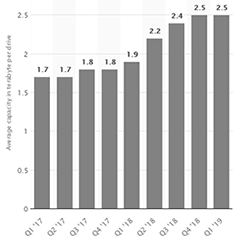
\includegraphics{fig4.png}}
\caption{Average capacity of Seagate hard disk drives (HDDs) worldwide from FY2017 to FY2019, by quarter (in terabyte per drive).}
\label{fig}
\end{figure}

This statistics revealed that the average capacity of \textit{Seagate} \textit{Hard Disk Drives} (\textit{HDDs}), at the first quarter of 2019 year was approximately 2.5 \textit{terabytes} per drive.

\vspace{4pt}

To see clearly, the increase of data and information, that can be kept in a \textit{qubit}, the following table illustrates a simple comparison of Quantum Values (\textit{SuperDense Coding}, most precisely, \textit{Quantum Bits} vs. \textit{Classical Bits}):

\begin{table}[!hp]
\centering
    \caption{Comparison of Quantum Values (SuperDense Coding, most precisely, Quantum Bits vs. Classical Bits)}
    \begin{tabular}{ |p{1.8cm}|p{5.8cm}| }
     \hline
     \multicolumn{2}{|c|}{\textbf{\textit{Qubits (Quantum Bits)} vs. \textit{Bits}}} \\
     \hline
     \hline
     \textbf{\# Qubits} & \textbf{\# Bits}\\
     \hline
     \hline
     \textbf{1 qubit} & 2 bits \\
     \hline
     \textbf{2 qubits} & 4 bits \\
     \hline
     \textbf{3 qubits} & 8 bits = 1 byte \\
     \hline
     \textbf{4 qubits} & 16 bits \\
     \hline
     \textbf{5 qubits} & 32 bits \\
     \hline
     \textbf{6 qubits} & 64 bits \\
     \hline
     \textbf{7 qubits} & 128 bits \\
     \hline
     \textbf{8 qubits} & 256 bits \\
     \hline
     \textbf{9 qubits} & 512 bits \\
     \hline
     \textbf{10 qubits} & 1,024 bits \\
     \hline
     \textbf{13 qubits} & 8,192 bits $\approx$ 1 kilobyte \\
     \hline
     \textbf{23 qubits} & 8,388,608 bits $\approx$ 1 megabyte \\
     \hline
     \textbf{33 qubits} & 8,589,934,592 bits $\approx$ 1 gigabyte \\
     \hline
     \textbf{43 qubits} & 8,796,093,022,208 bits $\approx$ 1 terabyte \\
     \hline
     \textbf{44 qubits} & 17,592,186,044,416 bits $\approx$ 2 terabytes \\
     \hline
     \textbf{45 qubits} & 35,184,372,088,832 bits $\approx$ 4 terabytes \\
     \hline
     \textbf{50 qubits} & 1,125,899,906,842,624 bits $\approx$ \\ & $\approx$ 128 terabytes \\
     \hline
     \textbf{72 qubits} & 4,722,366,482,869,645,213,696 bits $\approx$ \\ & $\approx$ 536,870,912 terabytes $\approx$ \\ & $\approx$ 512 exabytes $\approx$ \\ & $\approx$ 0.5 zettabytes \\
     \hline
     \textbf{2,000 qubits} & $\approx$ 1.1481$\times$10$^{602}$ ‬bits $\approx$ \\ & $\approx$ 1.4351$\times$10$^{586}$ terabytes $\approx$ \\ & $\approx$ 1.4351$\times$10$^{579}$ exabytes $\approx$ \\ & $\approx$ 1.4351$\times$10$^{576}$ zettabytes $\approx$ \\ & $\approx$ 1.4351$\times$10$^{573}$ yottabytes $\approx$ \\ & $\approx$ 143,510,000,000$\times$10$^{562}$ yottabytes\\
     \hline
     \textbf{n qubits} & 2\textsuperscript{n} bits \\
     \hline
    \end{tabular}
\end{table}

\vspace{1pt}

So, in reference to the previously mentioned statistics collected from \textit{Dell's Statistica} and believing that, every person, worldwide, that have a \textit{conventional computer} (as a \textit{Desktop} or a \textit{Laptop}) with a \textit{Hard Disk Drive} of 2.5 \textit{terabytes} of capacity, at average. A \textit{Quantum Computer} with a \textit{Quantum chip} of 72 \textit{qubits} (like \textit{Google} claimed, in 2018) would be 214,748,364$\times$ more powerful than the most of the current globally used \textit{conventional computers}' computing processing capabilities.

\vspace{4pt}

In another perspective, which can be analysed, is also to think that was predicted that in 2016, the volume of the entire Internet in the world would be 1.3 zettabytes. The same \textit{Quantum chip} of 72 \textit{qubits} from \textit{Google} would represent almost half of this huge amount of data.

\vspace{4pt}

So, it's possible to imagine the processing power that a \textit{Quantum Computer}, as \textit{D-Wave's 2000Q} could have. A huge quantity of the problems that \textit{conventional computers} couldn't resolve at a reasonable time or couldn't resolve at all, would be resolved very easily and fast, at a linear or polynomial time.

\newpage

After understanding the previously principles about \textit{Quantum Computing} and \textit{Quantum Bits}, it's reasonable to say that \textit{Quantum Computing} may have some powerful applications in \textit{Computer Science} and \textit{Informatics} in a near future, in some areas as, \textit{Quantum Programming}, \textit{Quantum Processors}, \textit{Cloud-based Quantum Computing}, \textit{Quantum Networks}, \textit{Quantum Cryptography}, \textit{Quantum Machine Learning}, among many others.

\section{Quantum Computing in Internet's Security}

\subsection{How can Quantum Computing affect Cryptography and Cybersecurity?}

As was previously said, the \textit{Quantum Computing} can have a lot of applications in \textit{Computer Science} and \textit{Informatics}. In this article/paper, it will be focused just on its applications in \textit{Cryptography} and \textit{Cybersecurity} and some related concerns that it can, possibly, awake in the future.

\vspace{4pt}

The following table provides which of these encryption algorithms are breakable using current \textit{Quantum Computing}:

\begin{table}[!hp]
\centering
    \caption{Encryption Algorithms breakable from the current Quantum Computing}
    \begin{tabular}{ |p{3cm}|p{3cm}| }
     \hline
     \begin{center}\textbf{Encryption Algorithm}\end{center} & \begin{center}\textbf{Security against \textit{Quantum Computing}}\end{center}\\
     \hline
     \hline
     \multicolumn{2}{|c|}{\textbf{Asymmetric (Public and Private)}} \\
     \multicolumn{2}{|c|}{\textbf{Key Encryption}} \\
     \hline
     \hline
     \textit{\textbf{3DES}} & \textbf{Insecure} \\
     \hline
     \textit{\textbf{AES-128}} & \textbf{Insecure} \\
     \hline
     \textit{\textbf{AES-256}} & \textbf{Secure} \\
     \hline
     \hline
     \multicolumn{2}{|c|}{\textbf{Symmetric Key Encryption}} \\
     \hline
     \hline
     \textit{\textbf{RSA-1024}} & \textbf{Insecure} \\
     \hline
     \textit{\textbf{RSA-2048}} & \textbf{Insecure} \\
     \hline
     \textit{\textbf{RSA-4096}} & \textbf{Insecure} \\
     \hline
     \textit{\textbf{ECC-256}} & \textbf{Insecure} \\
     \hline
     \textit{\textbf{ECC-512}} & \textbf{Insecure} \\
     \hline
     \textit{\textbf{Diffie-Hellman}} & \textbf{Insecure} \\
     \hline
     \textit{\textbf{Elliptical Curve}} & \\\textit{\textbf{Diffie-Hellman}} & \textbf{Insecure} \\
     \hline
    \end{tabular}
\end{table}

\vspace{1pt}



\vspace{4pt}

\newpage


\begin{center}
    \thanks{
        \small{
            \textbf{Article/Paper made in \href{http://tug.org/}{\TeX\,} \\
            for the course of\\
            \href{https://sites.google.com/campus.fct.unl.pt/aspi-2019}{\textit{Social-Professional\\Aspects of Informatics} (2018/2019)} of the\\
            \href{https://www.fct.unl.pt/en/education/course/integrated-master-computer-science}{\textit{Integrated Master of}\\
            \textit{Computer Science and Engineering}} at\\
            \href{https://www.fct.unl.pt/}{\textit{Faculty of Sciences and Technology of}\\
            \textit{New University of Lisbon}\\
            (\textit{FCT NOVA} - \textit{FCT/UNL})}}}
        }
\end{center}

\vspace{4pt}

\begin{center}
    \small{
        \textbf{
            This Article/Paper it's hosted in the following \\ \href{https://github.com/}{\textit{GitHub}}'s Repository/Host Service hyperlink:
        }\\
        \vspace{3pt}
        - \href{https://github.com/rubenandrebarreiro/quantum-computing-security-and-privacy-of-users}{https://github.com/rubenandrebarreiro/quantum-computing-security-and-privacy-of-users}
    }
\end{center}

\end{document}
